\documentclass[crop,tikz]{standalone}
\usetikzlibrary{positioning}
\begin{document}
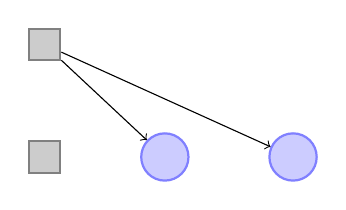
\begin{tikzpicture}
  [place/.style={circle,draw=blue!50,fill=blue!20,thick,
inner sep=0pt,minimum size=6mm}, transition/.style={rectangle,draw=black!50,fill=black!20,thick,
inner sep=0pt,minimum size=4mm}]
  \node[transition] (starting) {};
  \node[transition] (ending) [below=of starting] {};
  \node[place] (started) [right=of ending] {}
  edge [<-] (starting);
  \node[place] (another) [right=of started] {}
  edge [<-] (starting);

\end{tikzpicture}
\end{document}
